% intrinsic size and convergence correlations in weak lensing
% Basundhara Ghosh, Ruth Durrer, Bjoern Malte Schaefer

\documentclass[a4paper,fleqn,usenatbib]{mnras}
\usepackage[T1]{fontenc}
\usepackage{ae,aecompl}
\usepackage{graphicx}
\usepackage{amsmath}
\usepackage{amssymb}
\usepackage{txfonts}

\usepackage{float}
\usepackage{adjustbox}

\graphicspath{ {images/} }

\def\spirou#1{{\bf #1}}
\def\foca#1{{\bf #1}}
\def\basundhara#1{{\bf #1}}
\def\ruth#1{{\bf #1}}


% --- macros --- %
\newcommand{\icm}{intra-cluster medium}
\newcommand{\cmb}{cosmic microwave background}


% --- spirou's commands --- %
\newcommand{\ltsima}{$\; \buildrel < \over \sim \;$}
\newcommand{\lsim}{\lower.5ex\hbox{\ltsima}}
\newcommand{\gtsima}{$\; \buildrel > \over \sim \;$}
\newcommand{\gsim}{\lower.5ex\hbox{\gtsima}}
\newcommand{\bra}{\langle}
\newcommand{\ket}{\rangle}
\newcommand{\dang}{d_\mathrm{A}}
\newcommand{\dd}{\mathrm{d}}
\newcommand{\e}{\mathrm{e}}
\newcommand{\p}{\mathrm{p}}

\newcommand{\ci}{\mathrm{i}}
\newcommand{\vecx}{\bmath{x}}
\newcommand{\geo}{\vecx(\btheta,\chip)}
\newcommand{\vecl}{\bmath{\ell}}
\newcommand{\veclp}{\bmath{\ell}^\prime}
\newcommand{\trace}{\mathrm{tr}}
\newcommand{\dlp}{(\ell-\lprime)}

\newcommand{\chip}{{\chi^\prime}}
\newcommand{\chipp}{{\chi^{\prime\prime}}}
\newcommand{\lprime}{\ell^\prime}
\newcommand{\dirac}{\delta_D}
\newcommand{\likeli}{\mathcal{L}}
\newcommand\BG[1]{\textcolor{red}{#1}}

\onecolumn



% --- title --- %
\title[Intrinsic sizes and shapes of galaxies]
{Intrinsic and extrinsic correlations of galaxy shapes and sizes in weak lensing data}
\author[B. Ghosh, R. Durrer, B.M. Sch{\"a}fer]
{Basundhara Ghosh$^1$, Ruth Durrer$^1$, Bj{\"o}rn Malte Sch{\"a}fer$^2$\thanks{e-mail: bjoern.malte.schaefer@uni-heidelberg.de}\\
$^1$D{\'e}partment de la Physique Th{\'e}orique, Universit{\'e} de Gen{\`e}ve, 24 quai Ernest Ansermet, 1211 Gen{\`e}ve, Switzerland\\
$^2$Zentrum f{\"u}r Astronomie der Universit{\"a}t Heidelberg, Astronomisches Rechen-Institut, Philosophenweg 12, 69120 Heidelberg, Germany
}


% --- document --- %
\begin{document}
\pagerange{\pageref{firstpage}--\pageref{lastpage}}
\pubyear{2020}
\maketitle
\label{firstpage}


% --- abstract --- %
\begin{abstract}
The subject of this paper are shape and size correlations of galaxies due to weak gravitational lensing and due to direct tidal interaction of elliptical galaxies with gravitational fields sourced by the cosmic large-scale structure. Setting up a linear intrinsic alignment model for elliptical galaxies which parameterises the reaction of the galaxy to an external tidal shear field through the velocity dispersion, we predict intrinsic correlations and cross-correlations with weak lensing for both shapes and sizes, juxtaposing both types of spectra with lensing. We quantify the observability of the intrinsic shape and size correlations and estimate with the Fisher-formalism how well the alignment parameter can be determined from the Euclid weak lensing survey. Specifically, we find a contamination of the weak lensing convergence spectra with an intrinsic size correlation amounting to up to 10\%  over a wide multipole range $\ell=100\ldots300$, with a corresponding cross-correlation exhibiting a sign change, similar to the cross-correlation between weak lensing shear and intrinsic shapes. A determination of the alignment parameter yields a precision of a few percent forecasted for Euclid, and we show that all shape and many size correlations should be measurable with Euclid. 
\end{abstract}


% --- keywords --- %
\begin{keywords}
gravitational lensing: weak -- dark energy -- large-scale structure of Universe.
\end{keywords}


% --- section:  --- %
\section{introduction}\label{sect_intro}
Weak lensing has emerged as a powerful probe for investigating the cosmic large-scale structure \citep{mellier_probing_1999, bartelmann_weak_2001, amara_optimal_2007, bartelmann_gravitational_2010, kilbinger_cosmology_2015}, for testing gravitational theories and for constraining cosmological parameters. As gravitational lensing probes fluctuations in the gravitational potential directly \citep{kaiser_weak_1992, hu_weak_1999, hu_dark_2001, hu_dark_2002, bernstein_dark_2004, heavens_3d_2003,  heavens_measuring_2006, munshi_cosmology_2008, grassi_detecting_2014}, it depends on minimal assumptions and is fixed for a given gravitational theory. Correlations in the shapes of galaxies induced by weak lensing \citep{bernstein_shapes_2002, bernstein_comprehensive_2009} have been detected almost two decades ago, and by now lensing is recognised as a tool for investigating cosmological theories alongside the cosmic microwave background and galaxy clustering \citep{van_waerbeke_efficiency_1999, huterer_weak_2002, huterer_weak_2010, mortonson_dark_2013}. The last generation of surveys, most notably KiDS and DES \citep{Abbott:2017wau} have provided independent confirmation for the $\Lambda$CDM-model and support parameter determinations from the CMB, even though tensions between the two probes, most notably in the matter density $\Omega_m$ and $\sigma_8$ remain \citep{maccrann_cosmic_2014, douspis_tension_2019}. The next generation of surveys, in particular Euclid \citep{Amendola:2016saw} and LSST will probe cosmological models to almost fundamental limits of cosmic variance, but with decreasing statistical errors the control of systematical errors will become one of the central questions for data analysis, along with higher-order effects in the lensing signal related to evaluating the tidal shear fields along a geodesic \citep{Ghosh:2018nsm, thomas_relativistic_2014}, as well as non-Gaussian statistics of the lensing signal due to nonlinear structure formation and non-Gaussian contributions to the covariance \citep{jain_cosmological_1997, kayo_cosmological_2013, kayo_information_2013, munshi_tomography_2014}.

Among astrophysical contaminants of the weak lensing signal, intrinsic alignments \citep{jing_intrinsic_2002, mackey_theoretical_2002, heymans_weak_2004, altay_influence_2006, kirk_impact_2010, massey_origins_2013, kitching_limits_2016} are perhaps the most dramatic, leading to significant biases in the estimation of cosmological parameters, surpassing most likely baryonic corrections \citep{white_baryons_2004, semboloni_quantifying_2011}. There are two primary models for the two dominant galaxy types for linking the apparent shapes to tidal gravitational fields in the large-scale structure \citep{dubinski_cosmological_1992}, which acts, due to long-ranged correlations, as the medium to reduce randomness and to correlate the measured ellipticities. The shapes of spiral galaxies are thought to be determined by the orientation of the angular momentum of the stellar disc \citep{catelan_intrinsic_2001, crittenden_spin-induced_2001, bailin_internal_2005}, and ultimately of the dark matter halo harbouring the stellar component. With this idea in mind, shape correlations are traced back to angular momentum correlations, which in turn would depend through tidal torquing as the angular momentum generated mechanism on the tidal shear fields. Tidal torquing models commonly predict ellipticity correlations on small scales at a level of at most 10\% of the weak lensing signal on multipoles above $\ell\simeq300$ for a survey like Euclid, many physical assumptions have been challenged, most notably the orientation of the disc relative to the host halo angular momentum, as well as an over-prediction of the correlation inherent to the torquing mechanism.

Elliptical galaxies, on the other hand, are thought to acquire shape correlations through direct interaction with the tidal shear field \citep{schneider_halo_2010, blazek_separating_2012, merkel_intrinsic_2013, blazek_beyond_2017, tugendhat_angular_2018}: Second derivatives of the gravitational potential would give rise to an anisotropic deformation of the galaxy, in the principal directions of the tidal shear tensor. Interestingly, the reaction of a galaxy to the tidal shear field is determined by the inverse velocity dispersion $1/\sigma^2$ similar to lensing, where the relevant quantity is the gravitational potential in units of $c^2$. Tidal alignments of elliptical galaxies are thought to be present at intermediate angular scales of a few hundred in multipole $\ell$ for a survey like Euclid, with amplitudes being typically an order of magnitude smaller than that of the weak lensing effect. In parallel, alignment models using ideas from effective field theories provide parameterised relationships between tensors constructed from the cosmic density and velocity fields and can capture a wider range of alignment mechanisms and track them into the nonlinear regime \citep{vlah_eft_2019}, but perhaps with a less clear physical picture. There are indications that this in fact takes place in Nature, for instance in measurements of shape correlations in the local Universe \citep{brown_measurement_2002}, in shallow surveys \citep{lee_alignments_2007, chisari_cosmological_2013, pahwa_alignment_2016}, using stacking techniques or correlation techniques in deeper surveys \citep{hirata_galaxy-galaxy_2004, mandelbaum_wigglez_2011, chisari_intrinsic_2014} and correlation techniques in weak lensing surveys \citep{heavens_intrinsic_2000, heymans_weak_2003, kilbinger_dark-energy_2009, joachimi_constraints_2011, heymans_cfhtlens_2013, de_jong_kilo-degree_2013, jee_cosmic_2013, kilbinger_cfhtlens:_2013, schneider_galaxy_2013, kirk_cross-correlation_2015, joudaki_cfhtlens_2017, johnston_kids+gama:_2018}. Likewise, intrinsic alignment effects have been investigated in fluid-mechanical simulations of galaxy formation \citep[for instance][]{tenneti_galaxy_2014, tenneti_intrinsic_2015, chisari_intrinsic_2015, debattista_internal_2015, chisari_redshift_2016, hilbert_intrinsic_2016, hilbert_intrinsic_2017, bate_when_2019}.

While intrinsic alignments refer to a physical change of the appearance of the galaxies \citep[for reviews, see][]{kiessling_galaxy_2015, joachimi_galaxy_2015, kirk_galaxy_2015, troxel_intrinsic_2015}, there is an analogous deformation effect on the shape of the light bundle emanating from a galaxy by gravitational lensing. To lowest order, both effects depend on tidal gravitational field which suggests that the effects must be correlated. In fact, cross-correlations between the physical change in shape and the apparent change in shape are predicted to be nonzero for elliptical galaxies, and to be more exact, should in fact be negative as galaxies align themselves radially with a large structure while lensing generates a tangential alignment. As a result, ellipticity correlations of galaxies is a sum of the conventional weak lensing (often referred to as $GG$), the intrinsic alignment (or $II$) and the cross-correlation between the two (called $GI$). Parameter estimation from weak lensing \citep{casarini_non-linear_2011, capranico_intrinsic_2013, blazek_beyond_2017} as well as weak lensing mass reconstructions \citep{fan_intrinsic_2007, chang_dark_2017} would be affected by these intrinsic contributions, and can be taken care of by direct modelling or by self-calibration \citep{troxel_self-calibration_2012, yao_effects_2017, yao_self-calibration_2018, yao_separating_2019, pedersen_first_2019}. In addition, intrinsic alignments can show up in cross correlation with the reconstructed CMB-lensing deflection field \citep{hirata_cross-correlation_2004, hall_intrinsic_2014, chisari_contamination_2015, larsen_intrinsic_2016, merkel_imitating_2017}, and they might be usable as cosmological probes in their own right \citep{pandya_can_2019, taruya_improving_2020}.

There should be analogous effects of the size of an elliptical galaxy due to tidal gravitational fields: In gravitational lensing the light bundle can be isotropically enlarged, i.e. changed in size while the shape is conserved: This nonzero convergence is caused by the trace of the tidal shear field, and determines to lowest order magnification as well, adding cosmological information \citep{huff_magnificent_2011, takahashi_probability_2011}. Similarly, the size of an elliptical galaxy would physically change for a fixed velocity dispersion if the trace of the tidal shear field is nonzero, or equivalently, if it resides in an overdense or underdense region. An underdense region with density contrast $\delta < 0$ would source a gravitational potential $\Phi$ through the Poisson-equation $\Delta\Phi/c^2 = 3\Omega_m/(2\chi_H^2)\delta$, with the Hubble-distance $\chi_H = c/H_0$, such that the eigenvalues of $\partial_i\partial_j\Phi$ would be negative, stretching the galaxy to a physically larger size. Alternatively, one can argue that the change of volume (or area) is given by the Jacobian of the differential acceleration, i.e. of the tidal shear field, such that $V/V_0 = \mathrm{det}(\delta_{ab} + \partial_a\partial_b\Phi)$, implying that $\ln V-\ln V_0 = \ln\det(\delta_{ab} + \partial_a\partial_b\Phi) = \mathrm{tr}\ln(\delta_{ab} + \partial_a\partial_b\Phi) \simeq \mathrm{tr}(\partial_a\partial_b\Phi) = \Delta\Phi$ and consequently $V/V_0 = \exp(\Delta\Phi)$ and $(V-V_0)/V \simeq\Delta\Phi$. To what extend extrinsic and intrinsic size correlations can add to our understanding of cosmology has been investigated by \citet{heavens_combining_2013}.

The motivation of our paper are exactly these correlations between the sizes of elliptical galaxies as they would be predicted by a linear alignment model as a consequence of the trace $\Delta\Phi$ of the tidal shear tensor $\partial_a\partial_b\Phi$ being nonzero, as proposed by \citet{hirata_galaxy-galaxy_2004, hirata_intrinsic_2010}. These intrinsic size correlations would be generated in complete analogy to intrinsic shape correlations caused by the traceless part of the tidal shear, and would contaminate measurements of weak lensing convergence correlations \citep{alsing_weak_2014} in the same way as intrinsic shape correlations are a nuisance to the weak lensing shear. Alternatively, one can imagine these as a manifestation of ellipticity-density correlations \citep{hui_intrinsic/extrinsic_2002}, only that density is mapped out by the galaxy size. After introducing tidal interactions of elliptical galaxies with their surrounding large-scale structure in Sect.~\ref{sect_tidal}, we compute shape correlations from direct tidal interaction and through gravitational lensing in Sect.~\ref{sect_spectra}. We quantify the information content of each of the correlations and the amount of covariance in Sect.~\ref{sect_fisher}, before discussing our results in Sect.~\ref{sect_summary}. In general we work in the context of a $w$CDM-cosmology with a constant equation of state value of $w$ close to $-1$, and standard values for the cosmological parameters, i.e. $\Omega_m = 0.3$, $\sigma_8 =  0.8$, $h = 0.7$ and $n_s = 0.96$, and a parameterised spectrum for nonlinearly evolving scales. We compute numerical results on the information content of size-correlations for the case of a tomographic weak lensing survey like Euclid's \citep{Amendola:2016saw}. Throughout the paper, summation convention is implied.


% --- section:  --- %
\section{tidal interactions of galaxies and gravitational lensing}\label{sect_tidal}
In a simplified way one can imagine elliptical galaxies as a stellar component in virial equilibrium with a velocity dispersion $\sigma^2$, filling the gravitational potential. \citet{piras_mass_2018} then argue that if the velocity dispersion is isotropic, one can invoke the Jeans-equation for stationary and static systems in order to relate density $\rho(r)$ and potential $\Phi(r)$,
\begin{equation}
\sigma^2\partial_r\ln\rho(r) = -\partial_r\Phi
\quad\rightarrow\quad
\rho(r) \propto \exp\left(-\frac{\Phi(r)}{\sigma^2}\right),
\end{equation}
reminiscent of the barometric formula. If the gravitational potential is distorted by external fields as the galaxy is not an isolated object, the equipotential contours get distorted correspondingly and the stellar component reacts and galaxy assumes a different shape. To lowest order, the change in shape takes place along the principal axes of the tidal shear tensor $\partial_a\partial_b\Phi$, which is defined as the tensor of second derivatives of the gravitational potential $\Phi$,
\begin{equation}
\Phi(r) \rightarrow \Phi(r) + \frac{1}{2}\partial_a\partial_b\Phi\:r_a r_b,
\end{equation}
leading to a distortion of the density of the stellar component. For weak tidal fields, the exponential can be Taylor-expanded to yield
\begin{equation}
\rho \propto 
\exp\left(-\frac{\Phi(r)}{\sigma^2}\right)\left[1-\frac{\partial_a\partial_b\Phi}{2\sigma^2}r_a r_b\right].
\end{equation}
For this perturbed stellar component one can compute the change of the second moments of the brightness distribution, where we ignore projection effects for a moment and use $\rho(r)$ for projected quantities,
\begin{equation}
\Delta q_{cd} = 
\int\dd^2r\:\rho(r)\: r_c r_d\: r_a r_b\times\frac{\partial_a\partial_b\Phi}{2\sigma^2} = S_{abcd}\:\Phi_{ab},
\end{equation}
which bears a resemblance to the generalised Hooke-law $\Delta q_{cd} = S_{abcd}\:\Phi_{ab}$, relating the stresses $\Phi_{ab}$ to the observable strains $\Delta q_{cd}$, which suggests to think of $S_{abcd}$ as the susceptibility of a galaxy to change its shape or size under the influence of tidal gravitational fields. In the theory of elastic media one would then in fact use index symmetries to derive that there must be two material constants, similarly, in the theory of viscous fluids one defines two Lam{\'e}-viscosity coefficients (bulk and shear viscosity), so naturally the question arises whether the same constant of proportionality determines the size and the shape deformation as in the case of lensing.

In our model we assume that the reaction of the galaxy to the tidal shear is instantaneous, which is an assumption that can be challenged: Adjustment to a new tidal shear field should take place on the free-fall time scale $t_\mathrm{ff} = 1/\sqrt{G\rho}$ with the total matter density $\rho$, that is typically a factor of $\Delta = 200$ higher than the background density $\Omega_m\rho_\mathrm{crit}$ with $\rho_\mathrm{crit} = 3H_0^2/(8\pi G)$. Substitution shows tha the free fall time scale is only $\sqrt{8\pi/(3\Omega_m\Delta)}\simeq 0.37$ times shorter than the age of the Universe $1/H_0$, but because at least in linear structure formation tidal gravitational fields are close to constant in dark energy-cosmologies, the approximation might not be too bad. Of course in nonlinear structure formation, the time-scale of evolution would be much shorter and could give rise to an interesting time evolution of intrinsic alignments even for elliptical galaxies \citep{lee_nonlinear_2007, schafer_galactic_2012, schmitz_time_2018} 

After introducing polar coordinates, assuming spherical symmetry for the unperturbed galaxy and writing $r_0=r\cos\phi$ and $r_1=r\sin\phi$ for the vector components, the elasticity tensor is in our case given by
\begin{equation}
S_{abcd} = 
\frac{1}{2\sigma^2}\int\dd r\:r^5\rho(r)\int\dd\phi\:\cos^{4-(a+b+c+d)}\phi\sin^{a+b+c+d}\phi,
\end{equation}
has 16 entries and is fully symmetric under index exchange. Absorbing the prefactor $\int\dd r\:r^5\rho(r)/(2\sigma^2)$ into an alignment parameter $D$, $S_{abcd}$ can only assume three different values, namely $S_{0000} = \int\dd\phi\:\cos^4\phi = S_{1111} = \int\dd\phi\:\sin^4\phi = 3\pi/4$, $S_{0001} = \int\dd\phi\:\cos^3\phi\sin\phi = S_{1110} = \int\dd\phi\:\cos\phi\sin^3\phi = 0$ and $S_{0011} = \int\dd\phi\:\cos^2\phi\sin^2\phi = \pi/4$. 

Introducing the four Pauli-matrices $\sigma^{(n)}_{ab}$ as the basis for the tidal shear $\partial_a\partial_b\Phi$,
\begin{equation}
\sigma^{(0)} = \left(
\begin{array}{cc}
+1 & 0 \\ 0 & +1
\end{array}
\right),~
\sigma^{(1)} = \left(
\begin{array}{cc}
+1 & 0 \\ 0 & -1
\end{array}
\right),~
\sigma^{(2)} = \left(
\begin{array}{cc}
0 & +1 \\ -1 & 0
\end{array}
\right),
\mathrm{~and~}
\sigma^{(3)} = \left(
\begin{array}{cc}
0 & +1 \\ +1 & 0
\end{array}
\right),
\end{equation}
one can determine the change in size $s$ that is introduced by a tidal field $\propto\sigma_{ab}^{(0)}$,
\begin{equation}
s = 
\frac{1}{2}\Delta q_{cd}\sigma^{(0)}_{cd} = 
\frac{1}{2}S_{abij}\sigma^{(0)}_{cd}\sigma^{(0)}_{ab} = 
\frac{1}{2}\left(S_{0000} + S_{0011} + S_{1100} + S_{1111}\right) = 
\pi,
\end{equation}
whereas the change in shape $\epsilon_+$ introduced by a tidal field $\Phi_{ab}\propto\sigma^{(1)}_{ab}$ would be
\begin{equation}
\epsilon_+ = 
\frac{1}{2}\Delta q_{cd}\sigma^{(1)}_{cd} = 
\frac{1}{2}S_{abij}\sigma^{(1)}_{cd}\sigma^{(1)}_{ab} = 
\frac{1}{2}\left(S_{0000} - S_{0011} - S_{1100} + S_{1111}\right) =
\frac{\pi}{2},
\end{equation}
or the change in shape $\epsilon_\times$ generated by the tidal field $\Phi_{ab}\propto\sigma^{(3)}_{ab}$,
\begin{equation}
\epsilon_\times = 
\frac{1}{2}\Delta q_{cd}\sigma^{(3)}_{cd} =
\frac{1}{2}S_{abij}\sigma^{(3)}_{cd}\sigma^{(3)}_{ab} = 
\frac{1}{2}\left(S_{0101} + S_{0110} + S_{1001} + S_{1010}\right) = 
\frac{\pi}{2},
\end{equation}
i.e. the changes in shape are only half as large as the change in size, analogously to the weak lensing convergence with $\Delta\psi = 2\kappa$, which implies as well that the same alignment parameter governs the shape and size distortions. With an assumption on the shape of the projected stellar density $\rho(r)$, for instance a S{\'e}rsic-profile \citep{sersic_influence_1963, graham_concise_2005},
\begin{equation}
\rho(r) \propto \exp\left(-b(n)\left[\left(\frac{r}{r_0}\right)^{1/n}+1\right]\right),
\label{eqn_sersic}
\end{equation}
it is possible to derive the scaling of ellipticity induced by the action of a tidal gravitational field, dominantly with the size of the galaxy but also with the S{\'e}rsic-index $n$. In eqn.~(\ref{eqn_sersic}), $r_0$ is the scale radius of the stellar component, and $b(n)\simeq 2n - 1/3$, approximatively \citep{de_vaucouleurs_recherches_1948}. Computing the relevant integral $\int\dd r\:r^5\rho(r)$ for a properly normalised density distribution $\int\dd^2r\:\rho(r) = 2\pi\int\dd r\:r\rho(r) = 1$ and using the definition of ellipticity $\epsilon$ as it would result from the second moments $q_{ab}$ of the normalised brightness distribution $I(r)$ which we equate to the stellar density $\rho(r)$,
\begin{equation}
\epsilon = \frac{q_{xx}-q_{yy}}{q_{xx}+q_{yy}} + 2\ci\frac{q_{xy}}{q_{xx}+q_{yy}},
\quad\mathrm{with}\quad
q_{ab} = \int\dd^2 r\:\rho(r)\:r_a r_b,
\end{equation}
where one recognises the size of the image in the denominator, $q_{xx} + q_{yy} = \int\dd^2r\:\rho(r)(x^2+y^2) = 2\pi\int\dd r\:r^3\rho(r)$, it is possible to show the scaling of the ellipticity to be
\begin{equation}
\epsilon \propto 
\left(\int_0^\infty\dd r\:r^5\rho(r)\right) \Bigg/ \left(\int_0^\infty\dd r\:r^3\rho(r)\right) = 
r_0^2 \times \int_{-b}^\infty\dd x\:\left(\frac{x}{b}+1\right)^{6n-1}\exp(-x) \Bigg/ \int_{-b}^\infty\dd x\:\left(\frac{x}{b}+1\right)^{4n-1}\exp(-x).
\end{equation}
Technically, we obtained this result after substitution $x = b\left[(r/r_0)^{1/n}-1\right]$, where the ratio of integrals has in general only a numerical solution and shows the dependence of the susceptibility to shape change due to tidal forces caused by the distribution of the stars inside the galaxy. The dominant scaling of ellipticity with the size $r_0^2$ of the galaxy is dimensionally consistent with the linear tidal shear model $q_{ab} = S_{abcd}\:\Phi_{cd}$. The results are shown in Fig.~\ref{fig_sersic_scaling}, which indicates a strong scaling of the alignment parameter with increasing S{\'e}rsic-index $n$, where we should note that we consider the S{\'e}rsic-profile as a reasonably simple model for the stellar distribution, which is not consistent with a constant velocity dispersion $\sigma^2$, and neither a gravitating self-consistent solution. Rather, it is supposed to illustrate that the internal dynamics of an elliptical galaxy can impact on the magnitude of tidal alignment and that not all elliptical galaxies should have the same alignment parameter if their S{\'e}rsic-index varies.

\begin{figure}
\centering
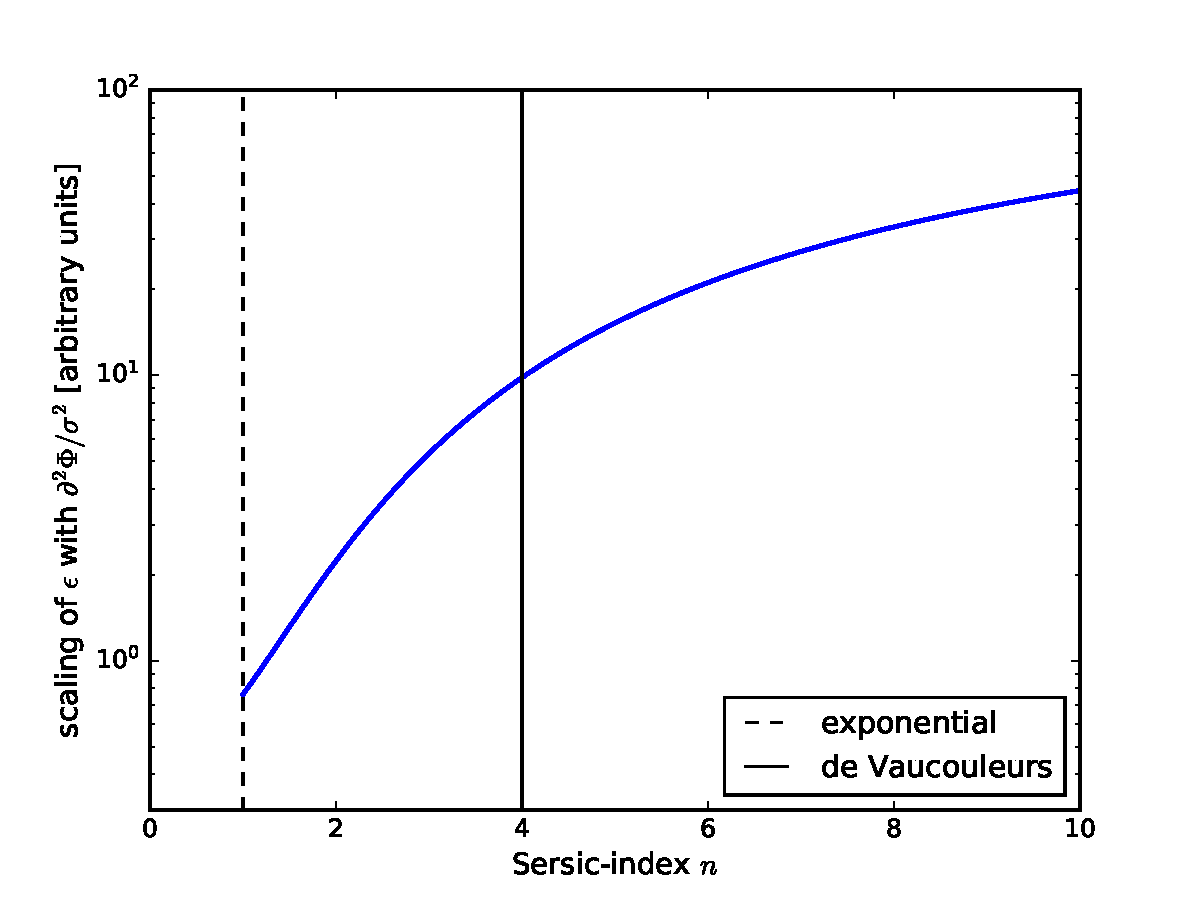
\includegraphics[scale=0.45]{./figures/sersic_scaling.pdf}
\caption{Scaling of the relation between ellipticity $\epsilon$ and S{\'e}rsic-index $n$, for a given tidal gravitational field and a given velocity dispersion $\sigma^2$. As particular cases, the exponential profile for $n=1$ and the de Vaucouleurs-profile for $n=4$ are indicated by vertical lines.}
\label{fig_sersic_scaling}
\end{figure}

It is straightforward to show that the distortion modes are all independent for the linear model, i.e. tidal fields $\propto\sigma^{(m)}_{ab}$ will never source distortion modes $\propto\sigma^{(n)}_{cd}$ with $m\neq n$. For making the influence of the tidal field on the galaxy size more specific, we compute the change in size $s$ explicitly as the second moment of the brightness distribution for the isotropic case,
\begin{equation}
s = 
\frac{1}{2\sigma^2}\int\dd^2r\:r^2\rho(r)\left[\frac{1}{2}\partial_a\partial_b\Phi\: r_ar_b\right] =
\frac{1}{2\sigma^2}\int\dd^2r\:r^2\rho(r)\left[\frac{1}{4}\Delta\Phi\:r^2\right] = 
\frac{\pi}{\sigma^2}\int r^5\dd r\:\rho(r)\frac{\Delta\Phi}{4} \propto \frac{\pi}{2}\Delta\Phi
\end{equation}
such that the change in size comes out proportional to the trace $\Delta\Phi$ of the tidal field and consistent with the above argumentation with the same definition of the alignment parameter $D$. 

With many galaxies in a tomographic bin $A$ with a suitable, normalised redshift distribution $p_A(z)\dd z$ one can define the line of sight-averaged ellipticity from second angular derivatives of the weighted projection of the potential $\Phi$:
\begin{equation}
\varphi_{A,ab} = \partial_a\partial_b\varphi_A
\quad\mathrm{with}\quad
\varphi_A = D\int\dd\chi\:p_A(z(\chi))\frac{\dd z}{\dd\chi}\frac{D_+}{a}\:\frac{\Phi}{\chi^2} = \int\dd\chi\:W_{\varphi,A}(\chi)\:\Phi,
\label{eqn_ia_los}
\end{equation}
with the Hubble-function $H(\chi)/c = \dd z/\dd\chi$ which originates from the transformation of the redshift distribution, and the growth rate $D_+/a$ of gravitational potentials, and the alignment parameter $D$, which encapsulates the proportionality between tidal shear and physical shape and size change. It would reflect the brightness distribution of a galaxy through its forth moments and scale inversely with the velocity dispersion $\sigma^2$. Because linear intrinsic alignments have the opposite sign compared to gravitational lensing in the same gravitational potential, we choose a negative value for the alignment parameter $D$ in order to not having to carry through minus-signs explicitly. This is due to the fact that an overdense region enlarges the image of a galaxy in lensing but compresses a galaxy physically.

Equation~(\ref{eqn_ia_los}) can be amended to include a bias model, as the galaxy density traces the dark matter density not perfectly. As the intrinsic shape and size-spectra correspond to ellipticity- and diameter-weighted galaxy correlation functions, a biasing model would in fact matter and can change the dependence between the observables and the tidal shear as a function of scale or redshift. For simplicity, we work with a bias of unity without any dependence on mass or redshift, which is reasonable for low-mass galaxies in the relevant redshift range \citep{sheth_large-scale_1999}. Modelling the statistics of the intrinsic alignment effects from a Gaussian random field as we do subsequently ignores that the galaxy shapes and sizes provide a measurement of the tidal field restricted to peak regions of the large-scale structure, which influences the statistics of tidal fields \citep{peacock_statistics_1985, schafer_galactic_2012}, while the dependence of tidal shears on the environment should be reproduced \citep{forero-romero_cosmic_2014, reischke_environmental_2018}.

The angular derivatives $\partial_a$ are related to the spatial derivatives $\partial_x$ through $\partial_a = \chi\partial_x$, with $x=\theta\chi$ in the small-angle approximation. From that, one can recover the ellipticity components $\epsilon_{+,A}$ and $\epsilon_{\times,A}$ as well as the size $s_A$ from a decomposition of the tensor $\varphi_{A,ab}$ with the Pauli-matrices $\sigma_{ab}^{(n)}$,
\begin{equation}
\varphi_{A,ab} = s_A\sigma^{(0)}_{ab} + \epsilon_{+,A}\sigma^{(1)}_{ab} + \epsilon_{\times,A}\sigma^{(3)}_{ab},
\end{equation}
where three components are sufficient because of the symmetry $\varphi_{A,ab} = \varphi_{A,ba}$. Using two properties of the Pauli-matrices $\sigma_{ab}^{(n)}$, namely $\sigma_{ab}^{(l)}\sigma_{bc}^{(m)} = \delta_{lm}\sigma^{(0)}_{ac} + \epsilon_{lmn}\sigma^{(n)}_{ac}$, and their tracelessness $\sigma^{(m)}_{aa} = 0$, it is possible to invert the last relation and to obtain the expansion coefficients,
\begin{equation}
s_A = \frac{1}{2}\varphi_{A,ab}\sigma^{(0)}_{ab},
\quad
\epsilon_{+,A} = \frac{1}{2}\varphi_{A,ab}\sigma^{(1)}_{ab},
\mathrm{~and}\quad
\epsilon_{\times,A} = \frac{1}{2}\varphi_{A,ab}\sigma^{(3)}_{ab}.
\end{equation}

The approach above is motivated by the weak lensing shear $\gamma$, which results from the tensor $\psi_{B,ij}$ containing the second derivatives of the weak lensing potential $\psi_B$,
\begin{equation}
\psi_{B,ij} = \partial_i\partial_j\psi_B
\quad\mathrm{with}\quad
\psi_B = 2\int\dd\chi\:\frac{G_B(\chi)}{\chi}\frac{D_+}{a}\Phi = \int\dd\chi\:W_{\psi,B}(\chi)\Phi,
\end{equation}
with the lensing efficiency
\begin{equation}
G_B(\chi) = \int_{\mathrm{max}(\chi,\chi_B)}^{\chi_{B+1}}\dd\chi^\prime\:p(\chi^\prime)\frac{\dd z}{\dd\chi^\prime}\left(1-\frac{\chi}{\chi^\prime}\right).
\end{equation}
It is interesting to note that the effect of convergence and shear are fully analogous to the changes in size and shape due to direct tidal interaction, up to two details: A light bundle, consisting of photons as relativistic test particles for the gravitational potential, is deflected twice as strongly compared to non-relativistic test particles such as the stars inside an elliptical galaxies, and the constant of proportionality that makes the gravitational potential dimensionless is $c^2$ in lensing instead of $\sigma^2$ for the intrinsic alignments. We will compute both lensing and intrinsic alignments from the dimensionless potential $\Phi$ give in units of $c^2$ and use a numerical value for the alignment parameter scaled by $c^2/\sigma^2$. Again, there is an analogous decomposition
\begin{equation}
\psi_{B,ij} = \kappa_B\sigma^{(0)}_{ij} + \gamma_{+,B}\sigma^{(1)}_{ij} +\gamma_{\times,B}\sigma^{(3)}_{ij}
\end{equation}
with the analogous inversion,
\begin{equation}
\kappa_B = \frac{1}{2}\psi_{B,ij}\sigma^{(0)}_{ij},
\quad
\gamma_{+,B} = \frac{1}{2}\psi_{B,ij}\sigma^{(1)}_{ij},
\mathrm{~and}\quad
\gamma_{\times,B} = \frac{1}{2}\psi_{B,ij}\sigma^{(3)}_{ij}.
\end{equation}
The intrinsic size field provides a measure of the projected density in the same way as the weak lensing convergence $\kappa$, but with a different weighting function:
\begin{equation}
s = 
\frac{1}{2}\varphi_{ab}\sigma^{(0)}_{ab} = 
\frac{D}{2}\sigma^{(0)}_{ab}\partial_a\partial_b\int\dd\chi\: p(\chi)\frac{D_+}{a}\frac{\Phi}{\chi^2} = 
\frac{D}{2}\int\dd\chi\:p(\chi)\frac{D_+}{a}\Delta\Phi = 
\frac{3\Omega_m}{4\chi_H^2}D\int\dd\chi\:p(\chi)\frac{D_+}{a}\delta,
\end{equation}
by substituting the Poisson-equation $\Delta\Phi = 3\Omega_m/(2\chi_H^2)\delta$, using $\partial_a = \chi\partial_x$ for the derivatives, and approximating the full Laplacian by the one containing the derivatives perpendicular to the line of sight. Again, one recognises a factor of two between the gravitational acceleration of photons in gravitational lensing and non-relativistic particles as in our case of stars inside an elliptical galaxy. As discussed before, an actual measurement of the mean size $s$ of the galaxies into a certain direction would in addition be weighted with a biasing factor because the tidal shear field is only measurable at positions where galaxies exist: While the inclusion of a reasonably simple linear and deterministic biasing model is certainly possible and straightforward, we ignore this out of simplicity. 

This implies that the statistics of all modes of the shape and size field can be described by spectra of the source fields, which in turn are given by a Limber-projection. Specifically, the spectrum of $\varphi_{A,ab}$ reads
\begin{equation}
\bra\varphi_{A,ab}(\bmath\ell)\varphi_{B,ij}^*(\bmath\ell^\prime)\ket = 
(2\pi)^2\dirac(\bmath\ell-\bmath\ell^\prime)\:C^{\varphi_A\varphi_B}_{abij}(\ell)
\quad\mathrm{with}\quad
C^{\varphi_A\varphi_B}_{abij}(\ell) = 
\ell_a\ell_b\ell_i\ell_j\:\int\frac{\dd\chi}{\chi^2}\:W_{\varphi,A}(\chi)W_{\varphi,B}(\chi)\:P_{\Phi\Phi}(k = \ell/\chi),
\end{equation}
similarly, one obtains for the the field $\psi_{B,ij}$,
\begin{equation}
\bra\psi_{A,ab}(\bmath\ell)\psi_{B,ij}^*(\bmath\ell\prime)\ket = 
(2\pi)^2\dirac(\bmath\ell-\bmath\ell^\prime)\:C^{\psi_A\psi_B}_{abij}(\ell)
\quad\mathrm{with}\quad
C^{\psi_A\psi_B}_{abij}(\ell) = 
\ell_a\ell_b\ell_i\ell_j\:\int\frac{\dd\chi}{\chi^2}\:W_{\psi,A}(\chi)W_{\psi,B}(\chi)\:P_{\Phi\Phi}(k = \ell/\chi),
\end{equation}
and finally for their cross-correlation,
\begin{equation}
\bra\varphi_{A,ab}(\bmath\ell)\psi_{B,ij}^*(\bmath\ell^\prime)\ket =
(2\pi)^2\dirac(\bmath\ell-\bmath\ell^\prime)\:C^{\varphi_A\psi_B}_{abij}(\ell)
\quad\mathrm{with}\quad
C^{\varphi_A\psi_B}_{abij}(\ell) =
\ell_a\ell_b\ell_i\ell_j\:\int\frac{\dd\chi}{\chi^2}\:W_{\varphi,A}(\chi)W_{\psi,B}(\chi)\:P_{\Phi\Phi}(k = \ell/\chi).
\end{equation}
In general, all lensing effects originating from a tidal gravitational field will have the opposite sign than the intrinsic tidal alignment, which causes the cross-correlation between lensing and intrinsic alignments to have a negative sign. This is taken care of numerically by choosing a negative value for the alignment parameter $D$, which does not affect the auto-correlations: Those are proportional to $D^2$ and therefore positive. In analogy we define the angular spectra $C^{\varphi_A\varphi_B}(\ell)$, $C^{\psi_A\psi_B}(\ell)$ and $C^{\varphi_A\psi_B}(\ell)$ of the potentials $\varphi_A$ and  $\psi_B$. For the spectrum of the gravitational potential we use a linear spectrum of the form $P_{\Phi\Phi}(k)\propto k^{n_s-4}T^2(k)$ with a transfer function $T(k)$ and a nonlinear extension on small scales \citep{cooray_power_2001, huterer_calibrating_2005}, normalised to $\sigma_8$, but assume Gaussian statistics throughout. We apply a smoothing on a scale defined through $M = 4\pi/3\:\Omega_m\rho_\mathrm{crit}R^3$, $\rho_\mathrm{crit} = 3H_0^2/(8\pi G)$, 
\begin{equation}
\Phi(k) \rightarrow \Phi(k)\exp\left(-\frac{(kR)^2}{2}\right),
\end{equation}
to the potential used for intrinsic alignments, where we set the mass scale to be $M=10^{12}M_\odot/h$: In doing this we can control how close size- and shape-correlations trace the tidal shear field, and select the relevant long-wavelength modes.


% --- section:  --- %
\section{Angular spectra of galaxy shapes and sizes}\label{sect_spectra}
The prefactors $\ell_a\ell_b$ appearing in the expressions for the spectra of the projected tidal shears can be compactly written by introducing polar coordinates, $\ell_0 = \ell\cos\phi$ and $\ell_1 = \ell\sin\phi$. Then,
\begin{equation}
\ell_a\ell_b = 
\frac{\ell^2}{2}\left(\sigma^{(0)}_{ab} + (\cos^2\phi-\sin^2\phi)\sigma^{(1)}_{ab} + 2\sin\phi\cos\phi\sigma^{(3)}_{ab}\right) = 
\frac{\ell^2}{2}\left(\sigma^{(0)}_{ab} + \cos(2\phi)\sigma^{(1)}_{ab} + \sin(2\phi)\sigma^{(3)}_{ab}\right),
\end{equation}
recovering the fact that the phase angle rotates twice as fast as the coordinate system. We are going to make the choice $\phi = 0$ by a suitable rotation of the coordinate frame, such that there are no contractions with $\sigma^{(3)}_{ab}$, and correspondingly vanishing $\gamma_\times$ or $\epsilon_\times$. This corresponds effectively to the computation of $E$- and $B$-modes of the shear field and of the ellipticity field, with
\begin{align}
e(\vecl) = &\hphantom{-}\cos(2\phi)\gamma_+(\vecl) + \sin(2\phi)\gamma_\times(\vecl),\\
b(\vecl) = &-\sin(2\phi)\gamma_+(\vecl) + \cos(2\phi)\gamma_\times(\vecl),
\end{align}
where in our model there are no $B$-modes due to the index exchange symmetry. Now, the decomposition with Pauli-matrices makes it possible to write down all ellipticity spectra as contractions of the the possible spectra of the source terms, for lensing,
\begin{equation}
C^{\gamma\gamma}_{AB}(\ell) = \frac{1}{4}\sigma^{(1)}_{ab}\sigma^{(1)}_{ij}C^{\psi_A\psi_B}_{abij}(\ell) = \frac{\ell^4}{4}C^{\psi_A\psi_B}(\ell),
\end{equation}
for intrinsic alignments,
\begin{equation}
C^{\epsilon\epsilon}_{AB}(\ell) = \frac{1}{4}\sigma^{(1)}_{ab}\sigma^{(1)}_{ij}C^{\varphi_A\varphi_B}_{abij}(\ell) = \frac{\ell^4}{4}C^{\varphi_A\varphi_B}(\ell),
\end{equation}
and for the cross-correlation between the two,
\begin{equation}
C^{\epsilon\gamma}_{AB}(\ell) = \frac{1}{4}\sigma^{(1)}_{ab}\sigma^{(1)}_{ij}C^{\varphi_A\psi_B}_{abij}(\ell) = \frac{\ell^4}{4}C^{\varphi_A\psi_B}(\ell).
\end{equation}
A measurement of the shape correlations is limited by a Poissonian shape noise contribution,
\begin{equation}
N_{AB}^\mathrm{shape}(\ell) = \sigma^2_\mathrm{shape}\frac{n_\mathrm{tomo}}{\bar{n}}\delta_{AB},
\end{equation}
with a value of $\sigma_\mathrm{shape} = 0.4$ and the number density $\bar{n} = 4.727\times 10^8$ galaxies per steradian typical for Euclid-studies. It is straightforward to show that of the 20 possible spectra 10 are in fact nonzero, and that certain consistency relations hold, for instance $\bra\kappa\kappa^\prime\ket = \bra\gamma_+\gamma_+^\prime\ket + \bra\gamma_\times\gamma_\times^\prime\ket$ as well as $\bra ss^\prime\ket = \bra\epsilon_+\epsilon_+^\prime\ket + \bra\epsilon_\times\epsilon_\times^\prime\ket$, in any coordinate frame.

The resulting extrinsic and intrinsic shape spectra are shown for a tomographic survey in Fig.~\ref{fig:shapeshape}: Intrinsic shape correlations are relevant at intermediate multipoles, but are surpassed by one to two orders of magnitude by weak lensing-induced shape correlations, for realistic values of the alignment parameter $D$. Intrinsic and extrinsic shapes are anti-correlated, and the cross-correlation is modulating the spectra over much wider multipole ranges. In fulfilment of the Cauchy-Schwarz-inequality, the cross-correlation has values between the pure lensing and intrinsic alignment effect. The alignment parameter $D$ was chosen to be $10^{-5}$, and scales proportional to $(c/\sigma)^2$, where $\sigma=10^5\mathrm{m}/\mathrm{s}$ would be a typical value for a Milky Way-sized object with $10^{12} M_\odot/h$: Increasing the velocity dispersion (where $\sigma\propto M^{1/3}$ due to the viral law) requires a larger alignment parameter $D$. This value of the alignment parameter is chosen lower than the value measured by \citet{tugendhat_angular_2018} in CFHTLenS-data, even though details of the models differ from a technical point of view \citep[][who compute the correlations in real-space before Fourier-transforming into Fourier-space, whereas our model is set up entirely in Fourier-space]{tugendhat_angular_2018}, the models themselves should be compatible. Compared to the IllustrisTNG-simulation \citep{Zjupa_tng_2020}, where the alignment parameter as a constant of proportionality is measured directly in the relation between ellipticity and tidal shear, our value for $D$ is higher, because the measurement of the ambient tidal shear field contains a contribution from the local matter density and disregards biasing effects. Currently, there are still large uncertainties concerning the value and its dependence on galaxy mass as well as a possible evolution in redshift and galaxy biasing, such that we decided to use an intermediate value. 

\begin{figure}
\centering
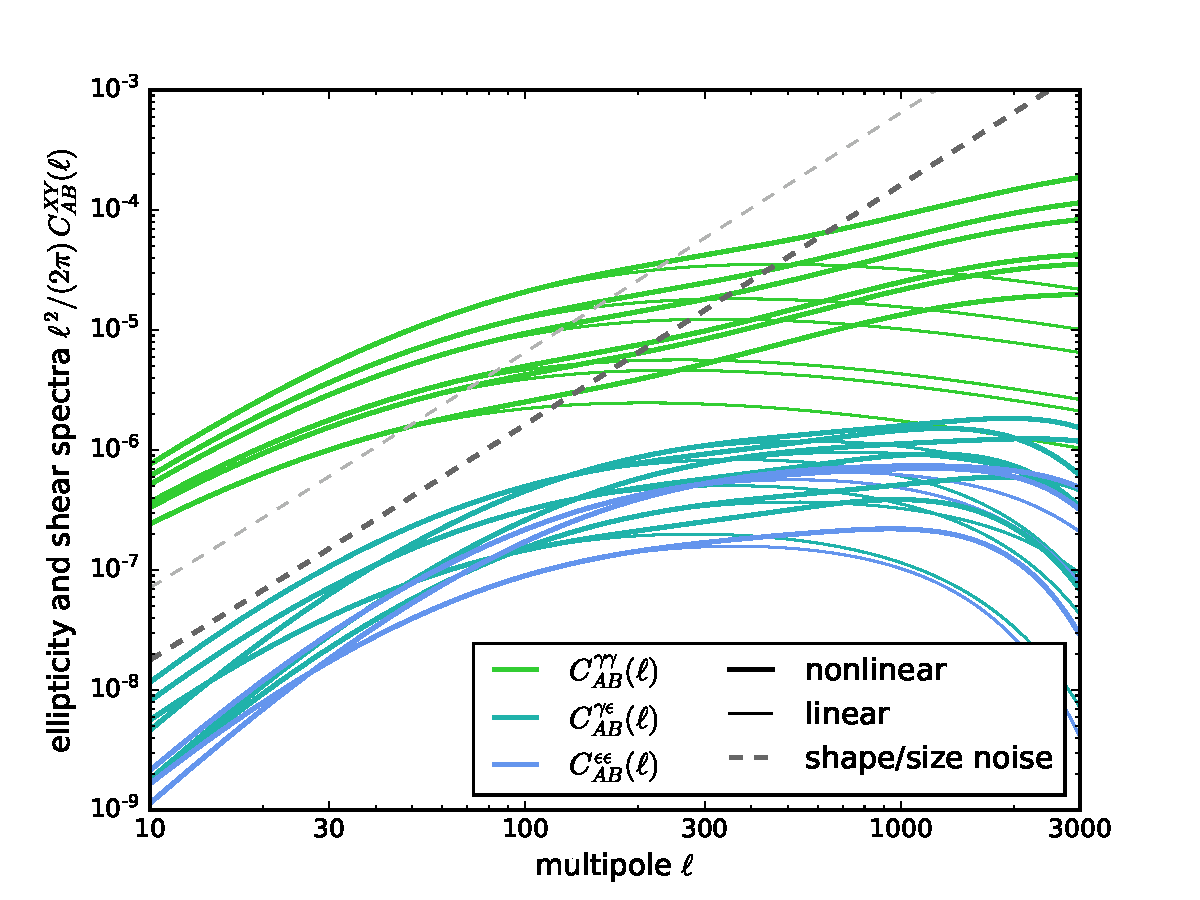
\includegraphics[scale=0.45]{./figures/ia_spectrum.pdf}
\caption{Shape-shape correlations as a function of multipole order $\ell$, separated by gravitational lensing $C_{AB}^{\gamma\gamma}(\ell)$, intrinsic size correlations $C_{AB}^{\epsilon\epsilon}(\ell)$ and the cross-correlation $C_{AB}^{\gamma\epsilon}(\ell)$ (of which we show the absolute value), with the Poissonian noise contributions $N_{AB}^\mathrm{shape}(\ell)$ (dark grey) and $N_{AB}^\mathrm{size}(\ell)$ (light grey, a factor of 4 higher) in comparison, for Euclid's redshift distribution and tomography with 3 bins, for a $\Lambda$CDM-cosmology with an alignment parameter $D=-10^{-5}$ on a mass scale $M = 10^{12}M_\odot/h$, corresponding to a virial velocity of $\sigma\simeq10^5\mathrm{m}/\mathrm{s}$. Thick and thin lines indicate a nonlinear and linear spectrum, respectively.}
\label{fig:shapeshape}
\end{figure}

In a similar manner as in the previous section, one obtains the size spectra from contracting the possible spectra of the source terms, for lensing,
\begin{equation}
C^{\kappa\kappa}_{AB}(\ell) = \frac{1}{4}\sigma^{(0)}_{ab}\sigma^{(0)}_{ij}C^{\psi_A\psi_B}_{abij}(\ell) = \frac{\ell^4}{4}C^{\psi_A\psi_B}(\ell),
\end{equation}
for intrinsic alignments,
\begin{equation}
C^{ss}_{AB}(\ell) = \frac{1}{4}\sigma^{(0)}_{ab}\sigma^{(0)}_{ij}C^{\varphi_A\varphi_B}_{abij}(\ell) = \frac{\ell^4}{4}C^{\varphi_A\varphi_B}(\ell),
\end{equation}
and again, for the cross-correlation between the two,
\begin{equation}
C^{s\kappa}_{AB}(\ell) = \frac{1}{4}\sigma^{(0)}_{ab}\sigma^{(0)}_{ij}C^{\varphi_A\psi_B}_{abij}(\ell) = \frac{\ell^4}{4}C^{\varphi_A\psi_B}(\ell),
\end{equation}
i.e. all size-spectra are equal to their shape-counterparts. In the estimation process, there is a constant, diagonal noise contribution
\begin{equation}
N_{AB}^\mathrm{size}(\ell) = \sigma^2_\mathrm{size} \frac{n_\mathrm{tomo}}{\bar{n}}\delta_{AB},
\end{equation}
with the size noise $\sigma_\mathrm{size} = 0.8$.

Fig.~\ref{fig:shapeshape} shows at the same time the intrinsic and extrinsic size-spectra, as they would result from a tomographic survey. In fact, as a consequence of the linear alignment model and the linearity of weak lensing the size-correlations are identical to the shape correlations, including the anti-correlation between intrinsic and extrinsic size. Given the fact that there is a slightly higher uncertainty in the measurement of angular size in comparison to shape one can already now expect that the corresponding signal to noise-ratios for size-correlations are slightly inferior to shapes. These statements rely on the fact that the same alignment parameter $D$ is relevant for both shapes and sizes, as the linear alignment model would suggest. Similarly, we show in Fig.~\ref{fig:pearson} the Pearson correlation coefficient $r_{\gamma\epsilon}$ as a function of multipole $\ell$,
\begin{equation}
r_{\gamma\epsilon} = \frac{C^{\gamma\epsilon}_{AA}(\ell)}{\sqrt{C^{\gamma\gamma}_{AA}(\ell)\: C^{\epsilon\epsilon}_{AA}(\ell)}},
\end{equation}
where we would like to emphasise that the Pearson-coefficients for shapes and sizes are identical, $r_{\gamma\epsilon}= r_{\kappa s}$. We set the bin-indices equal, $A = B$, because only in this case $C^{\epsilon\epsilon}_{AB}(\ell)$ and $C^{ss}_{AB}(\ell)$ are unequal to zero. The values for $r_{\gamma\epsilon}$ suggest that there is in fact redundancy in the spectra.

\begin{figure}
\centering
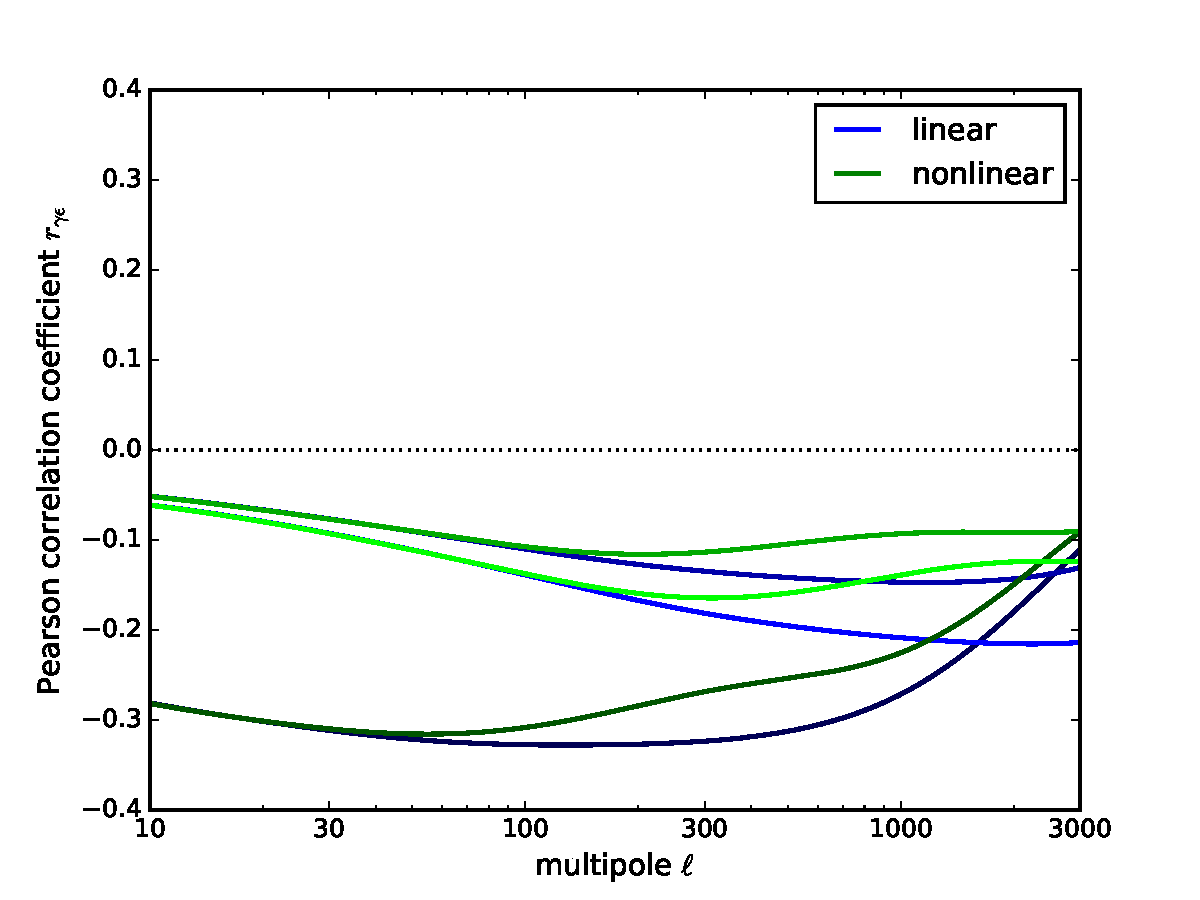
\includegraphics[scale=0.45]{./figures/pearson_coefficient.pdf}
\caption{Pearson correlation coefficients $r_{\gamma\epsilon}$ as a function of multipole order $\ell$.}
\label{fig:pearson}
\end{figure}

Finally, we compute the cross-correlations between galaxy shapes and sizes, for lensing
\begin{equation}
C_{AB}^{\kappa\gamma}(\ell) = \frac{1}{4}\sigma^{(0)}_{ab}\sigma^{(1)}_{ij}C^{\psi_A\psi_B}_{abij}(\ell) = \frac{\ell^4}{4}C^{\psi_A\psi_B}(\ell)
\end{equation}
for intrinsic alignments,
\begin{equation}
C_{AB}^{s\epsilon}(\ell) = \frac{1}{4}\sigma^{(0)}_{ab}\sigma^{(1)}_{ij}C^{\varphi_A\varphi_B}_{abij}(\ell) = \frac{\ell^4}{4}C^{\varphi_A\varphi_B}(\ell)
\end{equation}
and for the cross-correlation between lensing and alignments,
\begin{align}
C_{AB}^{\kappa\epsilon}(\ell) & = \frac{1}{4}\sigma^{(0)}_{ab}\sigma^{(1)}_{ij}C^{\psi_A\varphi_B}_{abij}(\ell) = \frac{\ell^4}{4}C^{\psi_A\varphi_B}(\ell)\\
C_{AB}^{s\gamma}(\ell) & = \frac{1}{4}\sigma^{(0)}_{ab}\sigma^{(1)}_{ij}C^{\psi_A\varphi_B}_{abij}(\ell) = \frac{\ell^4}{4}C^{\varphi_A\psi_B}(\ell),
\end{align}
where due to the independence of the errors in the shape and size correlations one does not have to deal with a noise contribution when estimating spectra. Effectively, the cross-correlations between shape and size look identical to the autocorrelations, but in their estimation process there is no noise term, if statistical independence of the two measurement processes for shape and size is given.


% --- section:  --- %
\section{information content of shape and size correlations}\label{sect_fisher}
For quantifying the information content of intrinsic size and shape correlations in comparison to weak lensing convergence and shear we use the Fisher-matrix formalism. Arranging the measurements of galaxy shapes and sizes into a data vector yields the data covariance matrix,
\begin{equation}
C =
\left(
\begin{array}{cc}
C^{\epsilon\epsilon}_{AB}(\ell) + 2C^{\epsilon\gamma}_{AB}(\ell) + C^{\gamma\gamma}_{AB}(\ell) + N^\mathrm{shape}_{AB} & 
C^{s\epsilon}_{AB^\prime}(\ell) + C^{s\gamma}_{AB^\prime}(\ell) + C^{\kappa\epsilon}_{AB^\prime}(\ell) + C^{\kappa\gamma}_{AB^\prime}(\ell) \\
C^{s\epsilon}_{A^\prime B}(\ell) + C^{s\gamma}_{A^\prime B}(\ell) + C^{\kappa\epsilon}_{A^\prime B}(\ell) + C^{\kappa\gamma}_{A^\prime B}(\ell) & 
C^{ss}_{A^\prime B^\prime}(\ell) + 2C^{s\kappa}_{A^\prime B^\prime}(\ell) + C^{\kappa\kappa}_{A^\prime B^\prime}(\ell) + N^\mathrm{size}_{A^\prime B^\prime}
\end{array}
\right)
\end{equation}
Given the similarities between the shape and size correlations allows to rewrite the covariance matrix as
\begin{equation}
C = \left(
\begin{array}{cc}
\frac{\ell^4}{4}\left(C^{\varphi_A\varphi_B}(\ell)+2C^{\varphi_A\psi_B}(\ell)+C^{\psi_A\psi_B}(\ell)\right) + N^\mathrm{shape}_{AB} & 
\frac{\ell^4}{4}\left(C^{\varphi_A\varphi_{B^\prime}}(\ell)+2C^{\varphi_A\psi_{B^\prime}}(\ell)+C^{\psi_A\psi_{B^\prime}}(\ell)\right)\\
\frac{\ell^4}{4}\left(C^{\varphi_{A^\prime}\varphi_B}(\ell)+2C^{\varphi_{A^\prime}\psi_B}(\ell)+C^{\psi_{A^\prime}\psi_B}(\ell)\right) & 
\frac{\ell^4}{4}\left(C^{\varphi_{A^\prime}\varphi_{B^\prime}}(\ell)+2C^{\varphi_{A^\prime}\psi_{B^\prime}}(\ell)+C^{\psi_{A^\prime}\psi_{B^\prime}}(\ell)\right) + N^\mathrm{size}_{A^\prime B^\prime}
\end{array}
\right),
\end{equation}
which is dangerously close to being singular, underlining the degeneracy between the shape- and size measurements. Already at this stage one should expect that a combined measurement of shear and size does not yield strong improvements of the signal to noise-ratio alone, and given the fact that the same potentials are involved with identical physical dependences on cosmology, resulting Fisher-matrices will be very similar. We use the Fisher-matrix formalism as a quick way to quantify the fundamental sensitivities and degeneracies, while noting that the non-Gaussian shape of the likelihood matters in most cases and that tools for dealing with non-Gaussian likelihoods analytically exist \citep{takada_impact_2009, sellentin_non-gaussian_2015}.

The Fisher-matrix $F_{\mu\nu}$ for a tomographic survey assumes the generic form
\begin{equation}
F_{\mu\nu} = f_\mathrm{sky}\sum_\ell\frac{2\ell+1}{2}\mathrm{tr}\left(C^{-1}\partial_\mu S\:C^{-1}\partial_\nu S\right)
\end{equation}
where we implicitly assume a full sky coverage by having independent Fourier-modes. Similarly, we define the signal to noise ratio $\Sigma$,
\begin{equation}
\Sigma^2 = f_\mathrm{sky}\sum_\ell\frac{2\ell+1}{2}\mathrm{tr}\left(C^{-1}S\:C^{-1}S\right),
\end{equation}
with the noiseless spectrum $S(\ell)$ of which the signal strength is sought. For the case of Euclid, we extend the summation over the multipoles from $\ell=10$ to $\ell=3000$, and we are assuming for simplicity a full-sky coverage with no correlations between different multipoles but scale down the signal subsequently with a sky coverage of $f_\mathrm{sky}$, which would be justified because most of the signal originates at small angular scales. We set the number of tomographic bins to $n_\mathrm{tomo} = 5$.

Clearly, not all galaxies are ellipticals for which the tidal alignment model would apply, but only a fraction of $q\simeq 1/3$ of them. Therefore, we compute two values for the signal to noise-ratio $\Sigma$: First, we weight the $GI$-type spectra by a factor $q$, and the $II$-type spectra by a factor $q^2$ relative to the $GG$-term, as lensing operates on all galaxies identically irrespective of their type. These numbers for $\Sigma$ would correspond estimates of the spectra from the full data set and indicate the level of significance by which the shape or size correlations are incompatible with a pure gravitational lensing model. Fig.~\ref{fig:s2n_all} quantifies the signal to noise-ratio $\Sigma$ for measuring intrinsic shape and intrinsic size correlations: We compute the signal to noise-ratio for a measurement of the $II$ and $GI$-terms in both shape- and size correlations in the presence of the full cosmic variance, which is dominated by gravitational lensing, i.e. by the $GG$-terms. As expected, lensing-induced shape correlations are measurable at a higher signal to noise-ratio compared to size correlations, but both are easily within the reach of Euclid. The signal to noise ratio suggests that $GI$-type terms are detectable in shape correlations and perhaps marginally in size correlations, and $II$-terms are marginally detectable, with intrinsic shape correlations being the least disappointing.

The inverse $\Sigma^{-1}$ of the signal to noise-ratio is at the same time the relative error $D/\sigma_D$ on the alignment parameter $D$, which suggests that measurements of the alignment parameter can be carried out the level of a few ten percent, so the investigation of trends with galaxy mass, type or redshift seem feasible. We have chosen a rather conservative value for $D$, nothing precludes the usage of a strategy to boost intrinsic alignments relative to lensing.

\begin{figure}
\centering
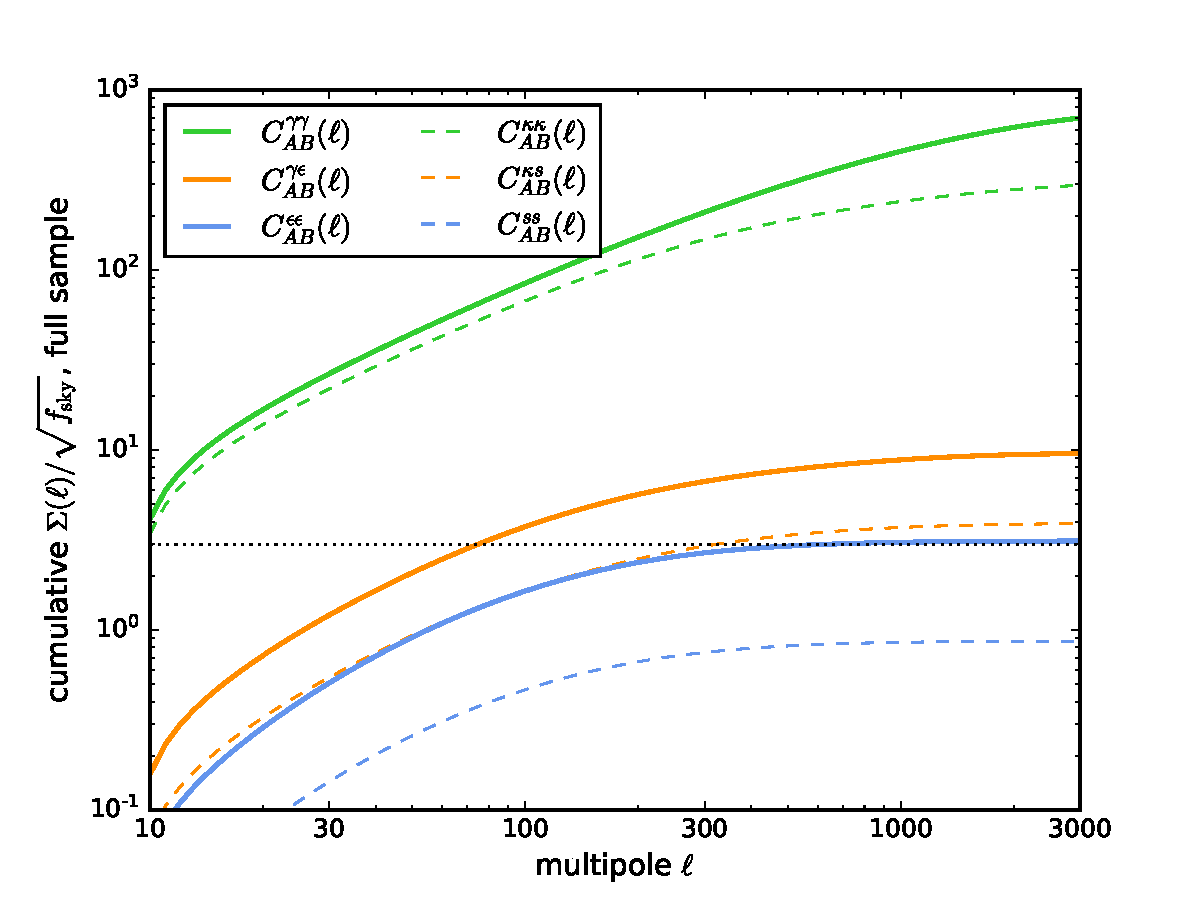
\includegraphics[scale=0.45]{./figures/sigma_all.pdf}
\caption{Cumulative signal to noise-ratio $\Sigma(\ell)/\sqrt{f_\mathrm{sky}}$ for Euclid 5-bin tomography for measuring shape correlations and intrinsic size correlations, for the full galaxy sample.}
\label{fig:s2n_all}
\end{figure}

On the other hand one could pursue the strategy to pre-select elliptical galaxies on the basis of their colours or morphologies and to measure the shape- and size correlations on the resulting, reduced data set. In this case, effectively, the total number of galaxies $\bar{n}$ is reduced by $q$ and the number of galaxy pairs by $q^2$, leading to an increased Poissonian noise term, which becomes larger by a factor of $q$. Consequently, the signal strength for weak lensing is much weaker, as it is estimated from a much smaller number of galaxies, but the relative amplitudes between lensing and the intrinsic alignment spectra are smaller. The resulting numbers are shown in Fig.~\ref{fig:s2n_elliptical}, where the overall higher shape and size noise terms decrease the significance, but vice versa, the amplitude of the intrinsic correlations relative to those of lensing are higher, such that a feasible strategy for measuring intrinsic shape correlations could be to measure the $GI$-terms and the $II$-terms with a selected sample of elliptical galaxies. The intrinsic size correlations, however, seem to be out of reach with Euclid, no matter the strategy. The attainable signal to noise ratio depends not only on the alignment parameter $D$ but also on the mass-scale on which the spectra are smoothed: The two are not independent and should be related through a virial relationship linking velocity dispersion $\sigma^2$ and mass $M$, $\sigma^2 \propto M^{2/3}$, but choosing a smaller mass scale has the consequence that higher multipoles contribute to the signal an increase $\Sigma(\ell)$.

\begin{figure}
\centering
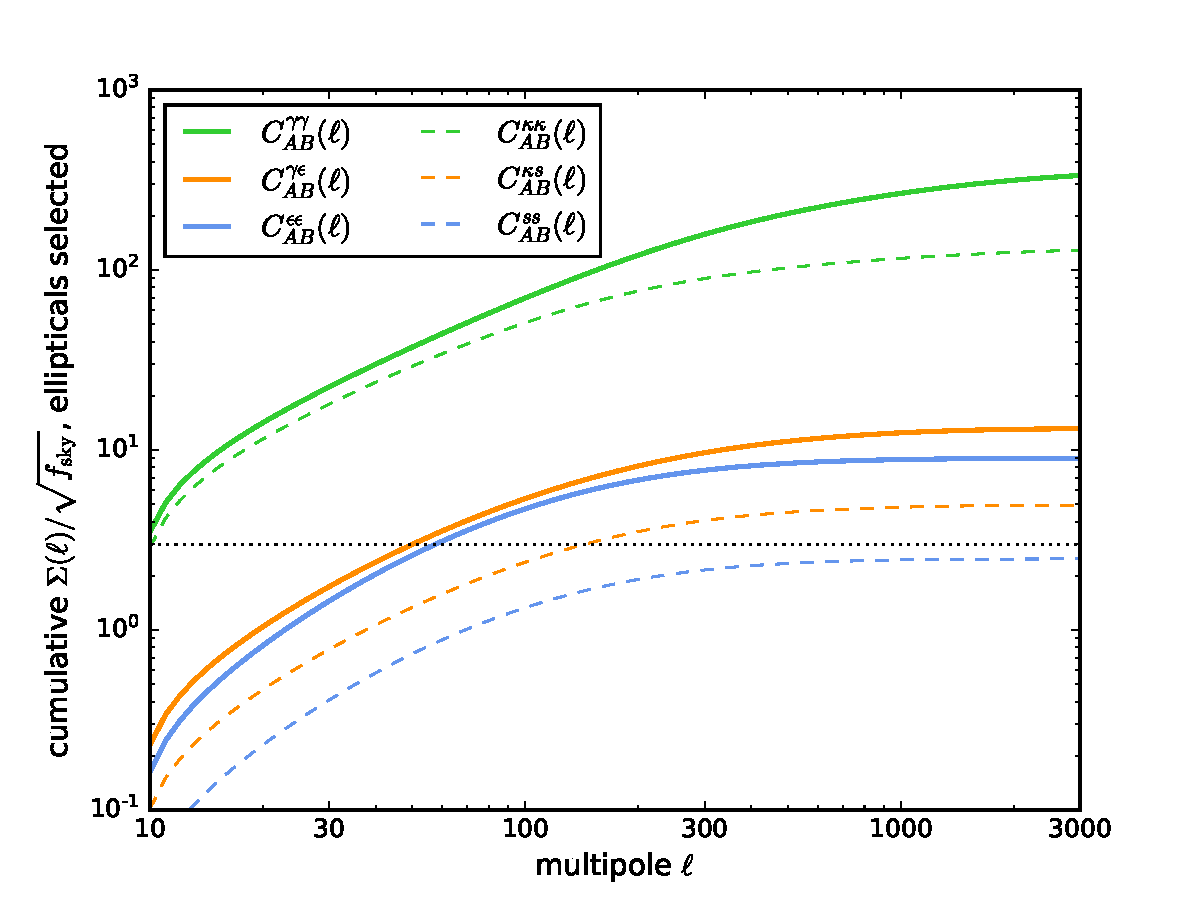
\includegraphics[scale=0.45]{./figures/sigma_elliptical.pdf}
\caption{Cumulative signal to noise-ratio $\Sigma(\ell)/\sqrt{f_\mathrm{sky}}$ for Euclid 5-bin tomography for measuring shape correlations and size correlations, for a case when elliptical galaxies are selected for the estimation of correlations.}
\label{fig:s2n_elliptical}
\end{figure}

Fig.~\ref{fig:fisher} shows constraints on a $w$CDM-cosmology from galaxy shapes and galaxy sizes: As both observables are probing tidal gravitational fields with identical physical dependences there can not be any fundamental difference in the degeneracies, with the only exception that the noise in the size-measurement is typically larger compared to the shape-measurement, which effectively cuts off high multipoles from contributing to the signal. And we would like to emphasise that the two measurements are highly correlated such that one does not gain an advantage from combining the two. We would argue, however, that there is potential to use shape and size-correlations to investigate deviations from the Newtonian form of the Poisson equation due to modified theories of gravity. For this, one needs a very good understanding of the detailed mechanisms of alignment with possibly nonlinear corrections to the tidal alignment model, as well as the scaling behaviour of the alignment parameter with redshift and galaxy mass \citep{hirata_intrinsic_2007}, and possibly different alignment parameters for subpopulations of elliptical galaxies, as the strong dependence on the S{\'e}rsic-index suggests. Fundamental degeneracies in the spectra 

\begin{figure}
\centering
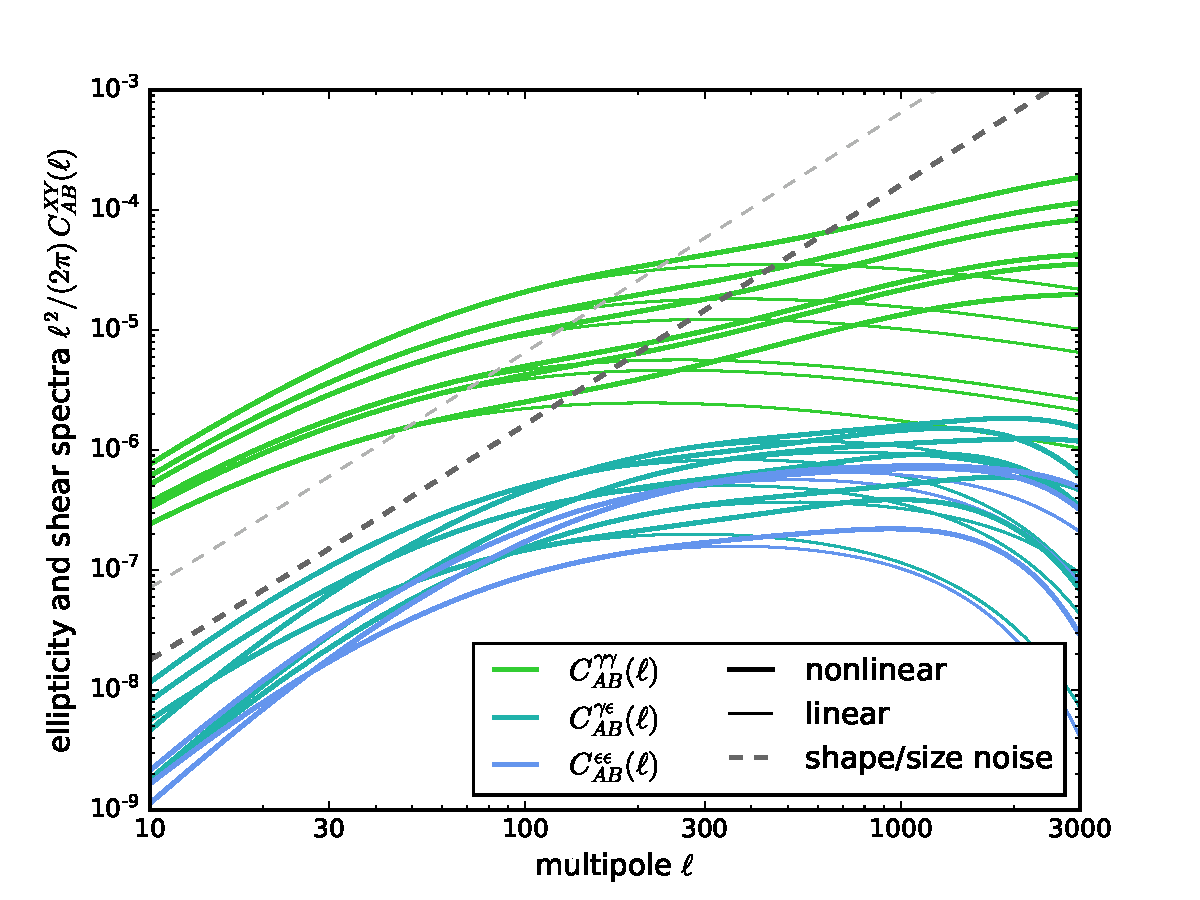
\includegraphics[scale=0.45]{./figures/ia_spectrum.pdf}
\caption{Marginalised $1\sigma$-contours from the Fisher-matrix analysis on a standard $\Lambda$CDM-parameter set, separated by $GG$, $GI$ and $II$-terms, for the shape correlations and the size correlations, with a fixed value of the alignment parameter $D$.}
\label{fig:fisher}
\end{figure}


% --- section: summary --- %
\section{summary}\label{sect_summary}
The subject of our investigation were extrinsic and intrinsic shape and size correlations of elliptical galaxies due to weak gravitational lensing and intrinsic alignments. Our starting point the description of the stellar density of a virialised system through the Jeans-equation, in which we perturb the gravitational potential with an external tidal shear field. Under the condition that this field is reasonably weak and the galaxy compact enough, one can compute that the response in shape and size of a galaxy is linear in the tidal shear field, and controlled by the galaxy's velocity dispersion $\sigma^2$. The susceptibility of a galaxy to tidal distortion is highly dependent on the stellar profile: A toy model using the S{\'e}rsic profile family showed a strong increase in the response from exponential profiles to de Vaucouleurs-profiles.

\begin{itemize}
\item{Assuming a weakly perturbed Jeans-equilibrium for elliptical galaxies naturally reproduces a linear response of the shape and the size of a galaxy to external tidal gravitational fields, and suggests that the same alignment parameter is responsible for the change in shape and in size. Nominally, the velocity dispersion $\sigma$ of the galaxy sets the scale for the gravitational field, which is remarkably similar to the quantity $\Phi/c^2$ in gravitational lensing. With virial equilibrium on can continue to argue that $\sigma^2$ is proportional to $M/R$ with the mass $M$ and the size $R$, such that the ratio $(R/\sigma)^2$, which controls the perturbation of the stellar component, is in fact constant \citep[compare][]{piras_mass_2018}. Therefore, alignments should not strongly depend on the mass scale under consideration, which would however enter through a convolution of the tidal shear spectrum with a filter function. Galaxy biasing would introduce an additional modulation of the intrinsic alignment effect and should be included in particular when comparing intrinsic alignment spectra with the straightforward galaxy clustering; in this sense the intrinsic shapes and sizes become weighted clustering spectra.}

\item{With a standard Poisson-equation it is the case that the galaxy sizes provide a direct mapping of the ambient matter density, and that the intrinsic and extrinsic shapes and sizes are consistent to each other. To which extend this can be used to probe deviations from Newtonian gravity is largely unclear and depends on a detailed understanding of the astrophysics of the objects. When using shape- and size-correlations as cosmological probes, the Poisson equation causes them to contain only degenerate information, and there is a direct mapping between $GG$, $GI$ and $II$-type terms. In addition, the shape and size-correlations are highly degenerate to the point where size correlations become redundant in comparison to the stronger and more sensitive shape correlations. We would like to make a point, however, that size correlations can provide an alternative method for mapping out the matter distribution.}

\item{Similar to the case of shape correlations, one obtains a completely diagonal autocorrelation for the intrinsic sizes, $C^{ss}_{AB}(\ell)\propto\delta_{AB}$ and a non-diagonal cross-correlation between size and convergence, $C^{s\kappa}_{AB}(\ell)$, so the non-diagonal part of the lensing signal only contains $GG$ and $GI$, but never $II$-terms \citep{jain_cross-correlation_2003, takada_tomography_2004, huterer_nulling_2005}, and in principle nulling- and boosting techniques \citep{joachimi_removal_2009, joachimi_controlling_2010, joachimi_intrinsic_2010} are applicable to size-correlations as well.}

\item{Computing a forecast for Euclid we obtain the result that intrinsic shape- and size-correlations as well as their cross-correlations with lensing are measurable. Typical signal to noise-ratios obtained for 5-bin tomography are with Euclid range around 10 for $C^{\gamma\epsilon}_{AB}(\ell)$- and $C^{\epsilon\epsilon}_{AB}(\ell)$-correlations, while size correlations are more difficult to detect. Simulating two strategies, measuring correlations in the full galaxy sample or pre-selecting elliptical galaxies first, showed that the latter could be able to make $C^{\epsilon\epsilon}_{AB}(\ell)$-correlations detectable. Our forecasts used a conservative value for the alignment parameter, $D\simeq -10^{-5}$, which should strongly depend on the mass scale \citep{piras_mass_2018} and potentially on the profile shape as well. Among the size correlations, $C^{\kappa s}_{AB}(\ell)$ could yield a marginal detection.}

\end{itemize}

In the future, we would like to investigate the usability of both types of shape and size spectra for designing specific tests of gravity, for instance for Vainshtein-type screening mechanisms \citep{kirk_optimising_2011, tessore_weak_2015}, which would manifest themselves in differences between the intrinsic and extrinsic shape and size spectra. Likewise, there is the question whether measurements of the velocity dispersion could help to disentangle intrinsic size from lensing shear, as the size effect would cause galaxies with the same velocity dispersion to appear systematically larger in underdense regions, and through velocity dispersion a common baseline could be established. In addition, we would like to point out that the susceptibility $\int\dd r\:r^5\rho(r)$ of a stellar system with density $\rho$ could differ for subclasses of elliptical galaxies giving rise to different effective alignment parameters $D$. Lastly, we would like to comment on possible intrinsic-size and shape effects arising at second order: Similar to lens-lens coupling one could expect a $B$-mode generation if lensing shear acts on a correlated intrinsic ellipticity field \citep[similar to][]{cooray_second-order_2002}, and if lensing deflection shifts the galaxies to new positions \citep{giahi_evolution_2013, giahi-saravani_weak_2014}. To what extent spiral galaxies would exhibit similar intrinsic size correlations is unclear, and possibly much more dependent on the astrophysics of galaxy formation, beyond models of tidal torquing \citep{schaefer_review:_2009}. Lastly we would argue that intrinsic size correlations are straightforward to be implemented in effective field theories of structure formation \citep{fang_fast-pt_2017, vlah_eft_2019}, as they only require the computation of $\Delta\Phi$ on a smoothed field.


% --- section: acknowledgements --- %
\section*{Acknowledgements}
BG thanks...   BMS likes to thank the Universidad del Valle in Cali, Colombia, for their kind hospitality. We thank Jolanta Zjupa for spotting a mistake in an early version of the draft.


% --- bibliography --- %
\bibliographystyle{mnras}
\bibliography{references}


\bsp
\label{lastpage}
\end{document}
